

\tikzset{every picture/.style={line width=0.75pt}} %set default line width to 0.75pt        

\begin{tikzpicture}[x=0.75pt,y=0.75pt,yscale=-1,xscale=1]
%uncomment if require: \path (0,446); %set diagram left start at 0, and has height of 446


%Shape: Rectangle [id:dp03411876837432981] 
\draw  [fill={rgb, 255:red, 30; green, 164; blue, 247 }  ,fill opacity=0.36 ] (13,60.03) -- (225.26,60.03) -- (225.26,233.73) -- (13,233.73) -- cycle ;
%Shape: Triangle [id:dp9375754488130867] 
\draw  [fill={rgb, 255:red, 208; green, 2; blue, 27 }  ,fill opacity=1 ] (126.3,74.43) -- (147.81,109.93) -- (104.79,109.93) -- cycle ;
%Shape: Ellipse [id:dp16442697541796703] 
\draw  [fill={rgb, 255:red, 74; green, 144; blue, 226 }  ,fill opacity=1 ] (133.47,142.08) .. controls (133.47,131.22) and (142.25,122.41) .. (153.07,122.41) .. controls (163.9,122.41) and (172.67,131.22) .. (172.67,142.08) .. controls (172.67,152.95) and (163.9,161.76) .. (153.07,161.76) .. controls (142.25,161.76) and (133.47,152.95) .. (133.47,142.08) -- cycle ;
%Shape: Ellipse [id:dp8929359456575365] 
\draw  [fill={rgb, 255:red, 74; green, 144; blue, 226 }  ,fill opacity=1 ] (23.52,142.08) .. controls (23.52,131.22) and (32.29,122.41) .. (43.12,122.41) .. controls (53.94,122.41) and (62.72,131.22) .. (62.72,142.08) .. controls (62.72,152.95) and (53.94,161.76) .. (43.12,161.76) .. controls (32.29,161.76) and (23.52,152.95) .. (23.52,142.08) -- cycle ;
%Shape: Triangle [id:dp7376655464767954] 
\draw  [fill={rgb, 255:red, 208; green, 2; blue, 27 }  ,fill opacity=1 ] (61.28,74.43) -- (82.8,109.93) -- (39.77,109.93) -- cycle ;
%Shape: Rectangle [id:dp12169534238909918] 
\draw  [fill={rgb, 255:red, 245; green, 166; blue, 35 }  ,fill opacity=1 ] (160.24,77.31) -- (199.44,77.31) -- (199.44,116.65) -- (160.24,116.65) -- cycle ;
%Shape: Rectangle [id:dp008860357027288712] 
\draw  [fill={rgb, 255:red, 245; green, 166; blue, 35 }  ,fill opacity=1 ] (165.02,173.27) -- (204.22,173.27) -- (204.22,212.62) -- (165.02,212.62) -- cycle ;
%Shape: Rectangle [id:dp9615704991146319] 
\draw  [fill={rgb, 255:red, 245; green, 166; blue, 35 }  ,fill opacity=1 ] (77.54,123.37) -- (116.74,123.37) -- (116.74,162.72) -- (77.54,162.72) -- cycle ;
%Shape: Triangle [id:dp3026521490627023] 
\draw  [fill={rgb, 255:red, 208; green, 2; blue, 27 }  ,fill opacity=1 ] (124.39,173.27) -- (145.9,208.78) -- (102.88,208.78) -- cycle ;
%Shape: Ellipse [id:dp47582021898019566] 
\draw  [fill={rgb, 255:red, 74; green, 144; blue, 226 }  ,fill opacity=1 ] (39.77,193.91) .. controls (39.77,183.04) and (48.55,174.23) .. (59.37,174.23) .. controls (70.2,174.23) and (78.97,183.04) .. (78.97,193.91) .. controls (78.97,204.77) and (70.2,213.58) .. (59.37,213.58) .. controls (48.55,213.58) and (39.77,204.77) .. (39.77,193.91) -- cycle ;
%Shape: Rectangle [id:dp29141062253976635] 
\draw  [fill={rgb, 255:red, 247; green, 204; blue, 30 }  ,fill opacity=0.36 ] (14.91,267.32) -- (227.17,267.32) -- (227.17,363.29) -- (14.91,363.29) -- cycle ;
%Shape: Ellipse [id:dp4851406617475926] 
\draw  [fill={rgb, 255:red, 74; green, 144; blue, 226 }  ,fill opacity=1 ] (100.96,301.39) .. controls (100.96,290.52) and (109.74,281.72) .. (120.56,281.72) .. controls (131.39,281.72) and (140.16,290.52) .. (140.16,301.39) .. controls (140.16,312.25) and (131.39,321.06) .. (120.56,321.06) .. controls (109.74,321.06) and (100.96,312.25) .. (100.96,301.39) -- cycle ;
%Shape: Triangle [id:dp1307613946933155] 
\draw  [fill={rgb, 255:red, 208; green, 2; blue, 27 }  ,fill opacity=1 ] (64.15,281.72) -- (85.66,317.22) -- (42.64,317.22) -- cycle ;
%Shape: Rectangle [id:dp35663833636935394] 
\draw  [fill={rgb, 255:red, 245; green, 166; blue, 35 }  ,fill opacity=1 ] (165.98,282.67) -- (205.18,282.67) -- (205.18,322.02) -- (165.98,322.02) -- cycle ;
%Straight Lines [id:da6673185348400361] 
\draw    (263.82,202.55) -- (298.82,202.5) ;
\draw [shift={(300.82,202.49)}, rotate = 179.91] [color={rgb, 255:red, 0; green, 0; blue, 0 }  ][line width=0.75]    (10.93,-3.29) .. controls (6.95,-1.4) and (3.31,-0.3) .. (0,0) .. controls (3.31,0.3) and (6.95,1.4) .. (10.93,3.29)   ;
%Straight Lines [id:da17452505371177662] 
\draw    (227,311.73) -- (263.54,312.73) ;
%Straight Lines [id:da19470043848262208] 
\draw    (226.21,138.72) -- (264.67,139.72) ;
%Straight Lines [id:da10397627231220286] 
\draw    (264.67,139.72) -- (263.54,312.73) ;
%Shape: Ellipse [id:dp8385531363983802] 
\draw  [fill={rgb, 255:red, 80; green, 227; blue, 194 }  ,fill opacity=0.49 ][dash pattern={on 4.5pt off 4.5pt}] (300.82,202.49) .. controls (300.82,169.48) and (341.79,142.71) .. (392.32,142.71) .. controls (442.86,142.71) and (483.82,169.48) .. (483.82,202.49) .. controls (483.82,235.51) and (442.86,262.28) .. (392.32,262.28) .. controls (341.79,262.28) and (300.82,235.51) .. (300.82,202.49) -- cycle ;
%Straight Lines [id:da2475999051951534] 
\draw    (483.82,202.49) -- (526.82,202.29) ;
\draw [shift={(528.82,202.28)}, rotate = 179.73] [color={rgb, 255:red, 0; green, 0; blue, 0 }  ][line width=0.75]    (10.93,-3.29) .. controls (6.95,-1.4) and (3.31,-0.3) .. (0,0) .. controls (3.31,0.3) and (6.95,1.4) .. (10.93,3.29)   ;
%Shape: Rectangle [id:dp03611177475200367] 
\draw  [fill={rgb, 255:red, 250; green, 128; blue, 114 }  ,fill opacity=0.69 ] (493.91,302.59) -- (664.82,302.59) -- (664.82,365.82) -- (493.91,365.82) -- cycle ;
%Shape: Triangle [id:dp8126894821695971] 
\draw  [fill={rgb, 255:red, 208; green, 2; blue, 27 }  ,fill opacity=1 ] (514.8,315.86) -- (530.82,345.28) -- (498.77,345.28) -- cycle ;
%Shape: Rectangle [id:dp7704102629126468] 
\draw  [fill={rgb, 255:red, 245; green, 166; blue, 35 }  ,fill opacity=1 ] (587.24,317.74) -- (611.82,317.74) -- (611.82,344.28) -- (587.24,344.28) -- cycle ;
%Shape: Ellipse [id:dp8221231723533802] 
\draw  [fill={rgb, 255:red, 74; green, 144; blue, 226 }  ,fill opacity=1 ] (540.96,331) .. controls (540.96,322) and (548.32,314.72) .. (557.39,314.72) .. controls (566.47,314.72) and (573.82,322) .. (573.82,331) .. controls (573.82,339.99) and (566.47,347.28) .. (557.39,347.28) .. controls (548.32,347.28) and (540.96,339.99) .. (540.96,331) -- cycle ;
%Shape: Ellipse [id:dp6362055661503672] 
\draw  [fill={rgb, 255:red, 74; green, 144; blue, 226 }  ,fill opacity=1 ] (623.82,330.78) .. controls (623.82,322.22) and (630.54,315.28) .. (638.82,315.28) .. controls (647.11,315.28) and (653.82,322.22) .. (653.82,330.78) .. controls (653.82,339.34) and (647.11,346.28) .. (638.82,346.28) .. controls (630.54,346.28) and (623.82,339.34) .. (623.82,330.78) -- cycle ;
%Rounded Rect [id:dp4276999307253777] 
\draw  [fill={rgb, 255:red, 189; green, 16; blue, 224 }  ,fill opacity=0.24 ][dash pattern={on 4.5pt off 4.5pt}] (530,180.88) .. controls (530,172.26) and (536.98,165.28) .. (545.6,165.28) -- (612.22,165.28) .. controls (620.84,165.28) and (627.82,172.26) .. (627.82,180.88) -- (627.82,227.68) .. controls (627.82,236.29) and (620.84,243.28) .. (612.22,243.28) -- (545.6,243.28) .. controls (536.98,243.28) and (530,236.29) .. (530,227.68) -- cycle ;
%Straight Lines [id:da16188474121366347] 
\draw    (580,303) -- (580.79,245.19) ;
\draw [shift={(580.82,243.19)}, rotate = 90.79] [color={rgb, 255:red, 0; green, 0; blue, 0 }  ][line width=0.75]    (10.93,-3.29) .. controls (6.95,-1.4) and (3.31,-0.3) .. (0,0) .. controls (3.31,0.3) and (6.95,1.4) .. (10.93,3.29)   ;
%Straight Lines [id:da6849788730551594] 
\draw    (628.41,200.78) -- (726.8,200.21) ;
\draw [shift={(728.8,200.2)}, rotate = 179.67] [color={rgb, 255:red, 0; green, 0; blue, 0 }  ][line width=0.75]    (10.93,-3.29) .. controls (6.95,-1.4) and (3.31,-0.3) .. (0,0) .. controls (3.31,0.3) and (6.95,1.4) .. (10.93,3.29)   ;
%Shape: Cube [id:dp37842381676395975] 
\draw  [fill={rgb, 255:red, 155; green, 155; blue, 155 }  ,fill opacity=1 ] (734,184.65) -- (753.01,165.64) -- (800.82,165.64) -- (800.82,209.99) -- (781.81,229) -- (734,229) -- cycle ; \draw   (800.82,165.64) -- (781.81,184.65) -- (734,184.65) ; \draw   (781.81,184.65) -- (781.81,229) ;
%Shape: Triangle [id:dp43155300544119535] 
\draw  [fill={rgb, 255:red, 208; green, 2; blue, 27 }  ,fill opacity=0.74 ] (757.82,196.64) -- (768.82,215.28) -- (746.77,215.28) -- cycle ;
%Shape: Ellipse [id:dp43711941013528444] 
\draw  [fill={rgb, 255:red, 74; green, 144; blue, 226 }  ,fill opacity=0.61 ] (756.68,174.96) .. controls (759.97,171.47) and (767.99,168.64) .. (774.59,168.64) .. controls (781.19,168.64) and (783.86,171.47) .. (780.57,174.96) .. controls (777.27,178.45) and (769.25,181.28) .. (762.66,181.28) .. controls (756.06,181.28) and (753.38,178.45) .. (756.68,174.96) -- cycle ;
%Shape: Rectangle [id:dp795789574341274] 
\draw  [fill={rgb, 255:red, 245; green, 166; blue, 35 }  ,fill opacity=0.55 ] (784.08,192.39) -- (796.82,180.28) -- (796.38,202.57) -- (783.65,214.67) -- cycle ;

% Text Node
\draw (291,9) node [anchor=north west][inner sep=0.75pt]   [align=left] {{\fontfamily{helvet}\selectfont {\Large Supervised Learning}}};
% Text Node
\draw (74.98,37.58) node [anchor=north west][inner sep=0.75pt]   [align=left] {Training Data};
% Text Node
\draw (92.3,368.7) node [anchor=north west][inner sep=0.75pt]   [align=left] {Labels};
% Text Node
\draw (40.7,330.4) node [anchor=north west][inner sep=0.75pt]  [font=\footnotesize] [align=left] {Triangle};
% Text Node
\draw (100.26,329.44) node [anchor=north west][inner sep=0.75pt]  [font=\footnotesize] [align=left] {Circle};
% Text Node
\draw (165.08,330.4) node [anchor=north west][inner sep=0.75pt]  [font=\footnotesize] [align=left] {Square};
% Text Node
\draw (330,166.4) node [anchor=north west][inner sep=0.75pt]    {$ \begin{array}{l}
\ \ \ \ \ f_{i}(\textcolor[rgb]{0.82,0.01,0.11}{\blacktriangle }) =\ \hat{y}\\
\mathcal{L}( y,\ \hat{y}) \ \rightarrow f_{i+1} \ 
\end{array}$};
% Text Node
\draw (312,112) node [anchor=north west][inner sep=0.75pt]   [align=left] {{\Large \faCog}};
% Text Node
\draw (341.98,114.58) node [anchor=north west][inner sep=0.75pt]   [align=left] { Model Training};
% Text Node
\draw (449,111) node [anchor=north west][inner sep=0.75pt]   [align=left] {{\Large \faCog}};
% Text Node
\draw (340,224) node [anchor=north west][inner sep=0.75pt]   [align=left] {{\footnotesize Learning algorithm}};
% Text Node
\draw (551.98,375.01) node [anchor=north west][inner sep=0.75pt]   [align=left] {Test Data};
% Text Node
\draw (520,121) node [anchor=north west][inner sep=0.75pt]   [align=left] {\begin{minipage}[lt]{86.42pt}\setlength\topsep{0pt}
\begin{center}
{\small Model }\\{\small Inference/Evaluation}
\end{center}

\end{minipage}};
% Text Node
\draw (533,182) node [anchor=north west][inner sep=0.75pt]   [align=left] {$\displaystyle f(\textcolor[rgb]{0.82,0.01,0.11}{\blacktriangle })$};
% Text Node
\draw (572,183) node [anchor=north west][inner sep=0.75pt]   [align=left] {{\scriptsize = Triangle?}};
% Text Node
\draw (535.82,209.28) node [anchor=north west][inner sep=0.75pt]   [align=left] {{\scriptsize \textcolor[rgb]{0.29,0.29,0.29}{evaluation metrics}}};
% Text Node
\draw (726.98,139.01) node [anchor=north west][inner sep=0.75pt]   [align=left] {Final Model};
% Text Node
\draw (692,237) node [anchor=north west][inner sep=0.75pt]   [align=left] {$\displaystyle f(\textcolor[rgb]{0.82,0.01,0.11}{\blacktriangle \ } /\textcolor[rgb]{0.29,0.56,0.89}{\bullet \ } /\textcolor[rgb]{0.96,0.65,0.14}{\blacksquare })\text{=\{label\}}$};


\end{tikzpicture}